%%%%%%%%%%%%%%%%%%%%%%%%%%%%%%%%%%%%%%%%%
% Masters/Doctoral Thesis 
% LaTeX Template
% Version 2.5 (27/8/17)
%
% This template was downloaded from:
% http://www.LaTeXTemplates.com
%
% Version 2.x major modifications by:
% Vel (vel@latextemplates.com)
%
% This template is based on a template by:
% Steve Gunn (http://users.ecs.soton.ac.uk/srg/softwaretools/document/templates/)
% Sunil Patel (http://www.sunilpatel.co.uk/thesis-template/)
%
% Template license:
% CC BY-NC-SA 3.0 (http://creativecommons.org/licenses/by-nc-sa/3.0/)
%
%%%%%%%%%%%%%%%%%%%%%%%%%%%%%%%%%%%%%%%%%

%----------------------------------------------------------------------------------------
%	PACKAGES AND OTHER DOCUMENT CONFIGURATIONS
%----------------------------------------------------------------------------------------

\documentclass[
12pt, % The default document font size, options: 10pt, 11pt, 12pt
oneside, % Two side (alternating margins) for binding by default, uncomment to switch to one side
english, % ngerman for German
onehalfspacing, % Single line spacing, alternatives: onehalfspacing or doublespacing
%draft, % Uncomment to enable draft mode (no pictures, no links, overfull hboxes indicated)
%nolistspacing, % If the document is onehalfspacing or doublespacing, uncomment this to set spacing in lists to single
%liststotoc, % Uncomment to add the list of figures/tables/etc to the table of contents
%toctotoc, % Uncomment to add the main table of contents to the table of contents
%parskip, % Uncomment to add space between paragraphs
%nohyperref, % Uncomment to not load the hyperref package
headsepline, % Uncomment to get a line under the header
%chapterinoneline, % Uncomment to place the chapter title next to the number on one line
%consistentlayout, % Uncomment to change the layout of the declaration, abstract and acknowledgements pages to match the default layout
]{MastersDoctoralThesis} % The class file specifying the document structure

\usepackage[utf8]{inputenc} % Required for inputting international characters
\usepackage[T1]{fontenc} % Output font encoding for international characters
\usepackage{todonotes}
\usepackage{mathpazo} % Use the Palatino font by default

%\usepackage[style=numeric]{biblatex} % Use the bibtex backend with the authoryear citation style (which resembles APA)
\usepackage[backend=bibtex,style=numeric]{biblatex}
\bibliography{main} 

\usepackage[autostyle=true]{csquotes} % Required to generate language-dependent quotes in the bibliography

%----------------------------------------------------------------------------------------
%	MARGIN SETTINGS
%----------------------------------------------------------------------------------------

\geometry{
	paper=a4paper, % Change to letterpaper for US letter
	inner=2.5cm, % Inner margin
	outer=3.8cm, % Outer margin
	bindingoffset=.5cm, % Binding offset
	top=1.5cm, % Top margin
	bottom=1.5cm, % Bottom margin
	%showframe, % Uncomment to show how the type block is set on the page
}

%----------------------------------------------------------------------------------------
%	THESIS INFORMATION
%----------------------------------------------------------------------------------------

\thesistitle{Developing an accessible interface for a secure mobile device} % Your thesis title, this is used in the title and abstract, print it elsewhere with \ttitle
\supervisor{Dr. David \textsc{Hobbs}} % Your supervisor's name, this is used in the title page, print it elsewhere with \supname
\cosupervisor{Dr. Paul \textsc{Gardner-Stephen}}
\examiner{} % Your examiner's name, this is not currently used anywhere in the template, print it elsewhere with \examname
\degree{Bachelor of Engineering (Computer and Network Systems) (Honours)} % Your degree name, this is used in the title page and abstract, print it elsewhere with \degreename
\author{Luke Canavan} % Your name, this is used in the title page and abstract, print it elsewhere with \authorname
\addresses{} % Your address, this is not currently used anywhere in the template, print it elsewhere with \addressname

\subject{Engineering} % Your subject area, this is not currently used anywhere in the template, print it elsewhere with \subjectname
\keywords{} % Keywords for your thesis, this is not currently used anywhere in the template, print it elsewhere with \keywordnames
\university{\href{https://www.flinders.edu.au/}{Flinders University}} % Your university's name and URL, this is used in the title page and abstract, print it elsewhere with \univname
\department{\href{https://www.flinders.edu.au/college-science-engineering}{College of Science and Engineering}} % Your department's name and URL, this is used in the title page and abstract, print it elsewhere with \deptname
\group{The Douglas Adams Institute For Implausible Linguistics} % Your research group's name and URL, this is used in the title page, print it elsewhere with \groupname
\faculty{\href{}{}} % Your faculty's name and URL, this is used in the title page and abstract, print it elsewhere with \facname

\AtBeginDocument{
\hypersetup{pdftitle=\ttitle} % Set the PDF's title to your title
\hypersetup{pdfauthor=\authorname} % Set the PDF's author to your name
\hypersetup{pdfkeywords=\keywordnames} % Set the PDF's keywords to your keywords
}

\begin{document}

\frontmatter % Use roman page numbering style (i, ii, iii, iv...) for the pre-content pages

\pagestyle{plain} % Default to the plain heading style until the thesis style is called for the body content

%----------------------------------------------------------------------------------------
%	TITLE PAGE
%----------------------------------------------------------------------------------------

\begin{titlepage}
\begin{center}

\vspace*{.06\textheight}
{\scshape\LARGE \univname\par}\vspace{1.5cm} % University name
\textsc{\Large Honours Thesis}\\[0.5cm] % Thesis type

\HRule \\[0.4cm] % Horizontal line
{\huge \bfseries \ttitle\par}\vspace{0.4cm} % Thesis title
\HRule \\[1.5cm] % Horizontal line
 
\begin{minipage}[t]{0.4\textwidth}
\begin{flushleft} \large
\emph{Author:}\\
{\authorname} % Author name - remove the \href bracket to remove the link
\end{flushleft}
\end{minipage}
\begin{minipage}[t]{0.4\textwidth}
\begin{flushright} \large
\emph{Supervisor:} \\
{\supname} % Supervisor name - remove the \href bracket to remove the link  

\vspace{10mm}

\emph{Co-Supervisor:} \\
{\cosupname}
\end{flushright}
\end{minipage}\\[3cm]
 
\vfill

\large \textit{\degreename}\\[0.3cm]
%%\groupname\\\deptname\\[2cm] % Research group name and department name
 
\vfill

{\large \today}\\[4cm] % Date
%\includegraphics{Logo} % University/department logo - uncomment to place it
 
\vfill
\end{center}
\end{titlepage}

%----------------------------------------------------------------------------------------
%	DECLARATION PAGE
%----------------------------------------------------------------------------------------

\begin{declaration}
\addchaptertocentry{\authorshipname} % Add the declaration to the table of contents
\noindent I, \authorname, declare that this thesis titled, \enquote{\ttitle} and the work presented in it are my own. I confirm that:

\begin{itemize} 
\item This work was done wholly while in candidature for a degree of \degreename.
\item This document is in accordance with the plagiarism policy of \univname.
\item Where any part of this thesis has previously been submitted for a degree or any other qualification at this University or any other institution, this has been clearly stated.
\item Where I have consulted the published work of others, this is always clearly attributed.
\item Where I have quoted from the work of others, the source is always given. With the exception of such quotations, this thesis is entirely my own work.
\item I have acknowledged all main sources of help.
\item Where the thesis is based on work done by myself jointly with others, I have made clear exactly what was done by others and what I have contributed myself.\\
\end{itemize}
 
\noindent Signed:\\
\rule[0.5em]{25em}{0.5pt} % This prints a line for the signature
 
\noindent Date:\\
\rule[0.5em]{25em}{0.5pt} % This prints a line to write the date
\end{declaration}

\cleardoublepage

%----------------------------------------------------------------------------------------
%	ABSTRACT PAGE
%----------------------------------------------------------------------------------------

\begin{abstract}
  \addchaptertocentry{\abstractname} % Add the abstract to the table of contents
	//
\end{abstract}

%----------------------------------------------------------------------------------------
%	ACKNOWLEDGEMENTS
%----------------------------------------------------------------------------------------

\begin{acknowledgements}
\addchaptertocentry{\acknowledgementname} % Add the acknowledgements to the table of contents
	I would like to thank my supervisor, \supname , for his guidance and meaningful support in my undertaking of this project. 
	I would also like to thank my co-supervisor, \cosupname , for his support and technical assistance.
\end{acknowledgements}

%----------------------------------------------------------------------------------------
%	LIST OF CONTENTS/FIGURES/TABLES PAGES
%----------------------------------------------------------------------------------------

\tableofcontents % Prints the main table of contents

\listoffigures % Prints the list of figures

%\listoftables % Prints the list of tables

%----------------------------------------------------------------------------------------
%	ABBREVIATIONS
%----------------------------------------------------------------------------------------

%\begin{abbreviations}{ll} % Include a list of abbreviations (a table of two columns)

%\textbf{LAH} & \textbf{L}ist \textbf{A}bbreviations \textbf{H}ere\\
%\textbf{WSF} & \textbf{W}hat (it) \textbf{S}tands \textbf{F}or\\

%\end{abbreviations}

%----------------------------------------------------------------------------------------
%	PHYSICAL CONSTANTS/OTHER DEFINITIONS
%----------------------------------------------------------------------------------------

%\begin{constants}{lr@{${}={}$}l} % The list of physical constants is a three column table

% The \SI{}{} command is provided by the siunitx package, see its documentation for instructions on how to use it

%Speed of Light & $c_{0}$ & \SI{2.99792458e8}{\meter\per\second} (exact)\\
%Constant Name & $Symbol$ & $Constant Value$ with units\\

%\end{constants}

%----------------------------------------------------------------------------------------
%	SYMBOLS
%----------------------------------------------------------------------------------------

%\begin{symbols}{lll} % Include a list of Symbols (a three column table)

%$a$ & distance & \si{\meter} \\
%$P$ & power & \si{\watt} (\si{\joule\per\second}) \\
%Symbol & Name & Unit \\

%\addlinespace % Gap to separate the Roman symbols from the Greek

%$\omega$ & angular frequency & \si{\radian} \\

%\end{symbols}

%----------------------------------------------------------------------------------------
%	DEDICATION
%----------------------------------------------------------------------------------------

%\dedicatory{For/Dedicated to/To my\ldots} 

%----------------------------------------------------------------------------------------
%	THESIS CONTENT - CHAPTERS
%----------------------------------------------------------------------------------------

\mainmatter % Begin numeric (1,2,3...) page numbering

\pagestyle{thesis} % Return the page headers back to the "thesis" style

% Include the chapters of the thesis as separate files from the Chapters folder
% Uncomment the lines as you write the chapters

% Chapter Template

\chapter{Introduction}\label{chapter:firstchapter} % Main chapter title

\label{Chapter1} % Change X to a consecutive number; for referencing this chapter elsewhere, use \ref{ChapterX}

%----------------------------------------------------------------------------------------
%	SECTION 1
%----------------------------------------------------------------------------------------

\section{Introduction}\label{sec:firstsection}

%% give some background on importance and relevance of universal design
%% explain issue that needs to be addressed using this concept
%% mention this is a new project

To increase the accessibility of the MEGAphone mobile device, this project aims to create a universally designed case for the current revision of the project.
The intention is to give enhanced telephony access to everyone, regardless of physical impairments. 
The term ‘Universal Design’ is a concept first coined by Ron Mace where “the design of products, environments, programmes and services to be usable by all people, to the greatest extent possible, without the need for adaptation or specialized design” (National Disability Authority, nd). 
Existing design principles developed by the Center for Universal Design at North Carolina State University (Story, 1998) will be adopted to help guide this project in the right direction.

This is a new project, which will require Autodesk 3D CAD modeling software (or equivalent) in order to successfully translate concept sketches into real tangible designs. 
Inclusive design practices will play a central role in the design process as the success of the final product depends on its ability to provide accessibility to all (regardless of age or disability). 
Universal Design is an iterative process and therefore must be at the centre of the design philosophy from the start (Newel et al., 2011). 
Additionally, this project will look into how UD can incorporate digital sovereignty so that users can not only have an accessible interface, but one that can be easily repaired, modified and controlled by them.

%\begin{figure}
%\begin{centering}
%\includegraphics[width=10cm,height=10cm,keepaspectratio]{Figures/dont-panic-e1534046233310.jpg}
%\caption{The Hitch Hiker's Guide To The Galaxy (not to be confused with \cite{Reference1}. Image Credit David Strine (License: CC0)}
%\label{fig:ThisFig}
%\end{centering}
%\end{figure}

%----------------------------------------------------------------------------------------
%	SECTION 2
%----------------------------------------------------------------------------------------
\section{Background on the MEGAphone}

%% how was this project formed, and who works on it
The ‘MEGAphone’ is a digitally sovereign mobile device created by Dr Paul Gardner-Stephen with the intent to promote digital sovereignty (MEGA65, 2020).
This project began when a trend was noticed in modern consumer electronics, in that they design their products with ‘planned obsolescence’ in mind. 
Gardner-Stephen believes that users should have the ability to repair or modify any aspect of their device without difficulty (Fahrplan Events Germany, 2019).

%% explain the purpose of FPGA, and security features
The MEGAphone incorporates the use of a field programmable gate-array (FPGA), a hardware programmable CPU designed to mimic a Commodore 64 processor. 
This removes the need for emulation as well as providing modern performance advancements partially due to eliminating the need for costly emulation.

% (Section \ref{sec:firstsection}).

%----------------------------------------------------------------------------------------
%	SECTION 3
%----------------------------------------------------------------------------------------

\section{Project Objectives}

The main objective of this project, as outlined in the thesis is to design a prototype case for the MEGAphone that follows the seven Universal Design (UD) principles established at the Universal Design branch of the North Carolina State University (Story, 1998). 
This thesis will also aim to document the process of design as well as any modifications to the design and why these changes were made. 
In terms of the research component, this thesis aims to address the relevance of UD in the design process as well as identifying how device sovereignty can be supported during this process. 
The desired output of this project as is documented will be a physical prototype of the MEGAphone case as well as software-side accessibility features for the MEGA65 operating system. 
A physical prototype of this project will allow for demonstration of the UD features.
 
%----------------------------------------------------------------------------------------
%	SECTION 4
%----------------------------------------------------------------------------------------

\section{Research Questions}

This thesis aims to answer multiple research questions:
    • What is the relationship between digital sovereignty and universal design?
    • Why is Universal Design important in the design of products today?
    • How can the MEGAphone device case be designed to support those with disabilities?
    • What are the effects of COVID-19 on digital sovereignty and how does that affect the MEGAphone?

%----------------------------------------------------------------------------------------
%	SECTION 5
%----------------------------------------------------------------------------------------

\section{Scope of Project}

This project includes development of computer-aided design chassis prototype as well as accessibility software, written in VHDL for the MEGA65 operating system. 
PCB design and manufacturing for device switches and adapters are also included in the scope of the project.

%----------------------------------------------------------------------------------------
%	SECTION 6
%----------------------------------------------------------------------------------------

\section{Layout of Thesis}

Chapter 1 addresses the aims of the project as well as the questions that this thesis aims to answer. 
Chapter 2 investigates the issues in design and sovereignty and how Universal Design helps to overcomes many of these issues. 
Chapter 3 focuses on the methods and tools used to design and manufacture the case and the accessibility software. 
Chapter 4 discusses the design process and the incremental changes made to the design toward a definitive prototype, followed by a discussion in regard to the outcome of the project. 
Chapter 5 provides concluding remarks as well as an evaluation of each revision of the case and the accompanying software.
% Chapter Template

\chapter{Literature Review} % Main chapter title

\label{Chapter2} % Change X to a consecutive number; for referencing this chapter elsewhere, use \ref{ChapterX}

%----------------------------------------------------------------------------------------
%	SECTION 1   % TARGET 2500 WORDS IN THIS CHAPTER
%----------------------------------------------------------------------------------------

\section{Overview}  
The aim of this literature review is to explain the importance of Universal Design and sovereignty in any design process as well as some insight into how this benefits all users. 
This is all linked back to the MEGAphone device, specifically, the work carried out by the author.

%----------------------------------------------------------------------------------------
%	SECTION 2
%----------------------------------------------------------------------------------------

\section{History of Universal Design}
%% start with origin of UD
%% COVID, relevant to sovereignty, manufacturing
Universal Design (UD) is a concept that was first coined by the founder of 'The Center for Universal Design', Dr Ronald Mace at NC State University in the United States\cite{ronald}.
This concept was developed as there was a clear need for inclusion in product design due to the sizable number of individuals with a disability or 'of old age' in the United States. %%find census on aus as well
In a paper dubbed, 'The Universal Design File'\cite{universalfile}, Story and others noted that due to the average lifespan being longer today than the beginning of the 20th century, due to better healthcare among other reasons.
They highlight that, with age,

One idea that is often confused with this concept is that the term, 'accessibility' is synonymous with 'disability' and this is not the case.
UD is a design method that was created to level the playing field by designing to reach the greater population, all ages and all abilities.
In a paper by Bringolf \cite{accessible}, she explains that as UD is still a relatively new concept, even today, it has generally been understood as designing for those with disabilities.
In Australia, a country with disability descrimination legislation (to protect people with disabilities), Bringolf notes that designers with this mindset will often design for this out of fear of litigation.
Bringolf observed that this creates an unhealthy approach to 'designing for all' which is what UD was originally created for. %% revise this, not sure it makes sense
This is why Bringolf wants to fight for the concept that UD is for everyone, and by extension this author also wishes to reiterate that idea looking at the development of this project deliverable. %%too meta?

%----------------------------------------------------------------------------------------
%	SECTION 3
%----------------------------------------------------------------------------------------

\section{Logistics of COVID-19}
%% discuss issues with supply in Australia due to COVID, need independence from imports
//

%----------------------------------------------------------------------------------------
%	SECTION 4
%----------------------------------------------------------------------------------------

\section{Mobile Device Accessibility}
%% talk about evolution of accessibility in mobile devices and discuss the problem with regard to the lack of accessibility supported
%% talk about how some mobile devices are being designed to include accessibility features and relate this all to sovereignty
Accessibility in mobile devices has in many ways been a part of the recipe from its introduction with features in a modern context such as vibration motors for alerts or text-to-speech for typing or reading content aloud.
However, as time has progressed, accessibility has slowly faded to the background to the point that modern mobile devices, commonly referred to as smartphones, have accessibility features that are far inferior to what they should be. %%does this flow well from first sentence?
A study by Law \cite{smartphone}, points out that there are a number of issues in regard to the lack of UD within the ICT industry.
He discusses a key note at the time of writing in that very few mobile devices have 'out of the box' functionality to provide users with vision impairment a platform in which to interact with the device. %%relate to present day
%% CONTINUE THIS

%-----------------------------------
%	SUBSECTION 1
%-----------------------------------

\subsection{Accessible Device A}
%% TALK ABOUT ACCESSIBLE DEVICES IN THESE SECTIONS
//

%-----------------------------------
%	SUBSECTION 2
%-----------------------------------

\subsection{Accessible Device B}
//

%----------------------------------------------------------------------------------------
%	SECTION 5
%----------------------------------------------------------------------------------------

\section{Software Accessibility}
//

%-----------------------------------
%	SUBSECTION 1
%-----------------------------------

\subsection{iOS}
//

%-----------------------------------
%	SUBSECTION 2
%-----------------------------------

\subsection{Android}
//

%-----------------------------------
%	SUBSECTION 3
%-----------------------------------

\subsection{Windows 10}
Windows 10 is an operating system developed by Microsoft for the x86 architecture released in July 2015.

%----------------------------------------------------------------------------------------
%	SECTION 6
%----------------------------------------------------------------------------------------

\section{Repairability}
//

%----------------------------------------------------------------------------------------
%	SECTION 7
%----------------------------------------------------------------------------------------

\section{Summary}
// 
% Chapter Template

\chapter{Method} % Main chapter title

\label{Chapter3} % Change X to a consecutive number; for referencing this chapter elsewhere, use \ref{ChapterX}

%----------------------------------------------------------------------------------------
%	SECTION 1   % TARGET 500 WORDS IN THIS CHAPTER
%----------------------------------------------------------------------------------------

\section{Hardware}

The Digilent Nexys DDR4 development board was available as an alternative to the Trenz Electronics TE0725 board housed within the MEGAphone PCB when said device is not available, given that the MEGAphone is based on the same architecture, with much of the same functionality.
Physical prototypes of the MEGAphone chassis are printed using the Ultimaker 2+ and Ultimaker S5 3D printers using PLA plastic at 0.15mm print resolution, with support.
Soldering kits and a soldering oven was provided by Flinders University for a new build of the MEGAphone device, used to present the case prototype.

%----------------------------------------------------------------------------------------
%	SECTION 2
%----------------------------------------------------------------------------------------

\section{Software}

The following sections list the software that was used to assist the development of this project along with justifications as to why they were chosen.

%-----------------------------------
%	SUBSECTION 1
%-----------------------------------

\subsection{LibreCAD}

LibreCAD is a free open source 2D design software that was used to sketch the initial concepts for the main project deliverable. 
This softwar, based on a fork from the free QCAD community version, was chosen due to its accessible nature and useable interface.

%-----------------------------------
%	SUBSECTION 2
%-----------------------------------

\subsection{Fusion 360}

The computer-aided design software chosen for the MEGAphone chassis project is Autodesk Fusion 360 as it is very capable as well as efficient in regard to resource consumption. 
Autodesk Inventor was originally considered as the definitive CAD program, however due to the concern of user sovereignty, Autodesk Fusion 360 was chosen as it is more accessible to individuals as it does not require potentially expensive licensing for recreational use. 
This is useful for users who might want to modify the device to fit a unique purpose and follows the intention of the MEGAphone project as accessible to users.
FreeCAD, a potential alternative would have arguably suited the sovereignty aspect far better, however due to not having a design history timeline at the time of selection, this option was diregarded.
Fusion 360 also benefitted from the ability to create and present an animation of the device during the final project seminar which all ran natively in the software, hence no requirement to import resources.

%-----------------------------------
%	SUBSECTION 3
%-----------------------------------

\subsection{KiCAD}

KiCAD is an open source eCAD software used in the printed circuit board (PCB) planning and designing process.
This software was chosen over alternatives with potentially expensive licensing costs for the end user such as Altium Designer or Autodesk Eagle.
KiCAD is a powerful software in its own right, and with extensive support from its community, it is competitive with Altium Designer, which is widely considered the industry standard.

%-----------------------------------
%	SUBSECTION 4
%-----------------------------------

\subsection{Xilinx Vivado}

To avoid the performance inefficiencies that come with processor emulation, the MEGAphone is entirely FPGA based, written in VHDL (Virtual Hardware Description Language), including the virtual accessible keyboard system for Jellybean switch input.
The accessible software features will be completely transparent to the MEGA65 operating system (OS), meaning that it will treat the input as if it were any perhipheral without needing to know that the switch exists.
Given that Xilinx develop the Artix-7 100T FPGA used in on the device, they are the sole proprietor and hence there are no alternatives to the Vivado software.
This is however, not a problem as the software is free for anyone to use, as the FPGA is where the cost is covered.

%----------------------------------------------------------------------------------------
%	SECTION 3
%----------------------------------------------------------------------------------------

\section{Manufacturing and Sourcing}

The following are a list of sourced parts for this project (excluding locally sourced parts):

\begin{itemize} 
    \item Printed circuit boards are sourced from PCBway.
    \item Electronic components are sourced from Digi-Key.
    \item Jellybean switches are sourced from Ablenet.
    \end{itemize}

%----------------------------------------------------------------------------------------
%	SECTION 4
%----------------------------------------------------------------------------------------

\section{Contributions}

This section lists contributors to this project as well as a brief outline of their contributions:

\begin{itemize} 
    \item Dr. David Hobbs; Academic supervisor for the project, provides feedback and expertise on iterations of the MEGAphone chassis project.
    \item Dr. Paul Gardner-Stephen; Academic co-supervisor, provides general feedback, also primarily responsible for the MEGA65 platform, research assistant for coding the accessible keyboard sub-system (view chapter 4.6)
    \item Lucas Moss; developed a revised PCB for the MEGAphone device based on the first revision by Damien Kleiss, which provides the constraints for the author's project.
    \item The author is responsible for designing the MEGAphone device chassis, accompanying PCBs including EZ access keys, Jellybean switch adapter and rocker switch array.
    \end{itemize}
% Chapter Template

\chapter{Development and Discussion} % Main chapter title

\label{Chapter4} % Change X to a consecutive number; for referencing this chapter elsewhere, use \ref{ChapterX}

%----------------------------------------------------------------------------------------
%	SECTION 1   % TARGET 6000 WORDS IN THIS CHAPTER
%----------------------------------------------------------------------------------------

\section{Overview}

The first revision of the prototype case is presented in this chapter.
Specifically, this section goes into detail about the process of designing as an iterative process where improvements and changes to the design are discussed and evaluated.


%----------------------------------------------------------------------------------------
%	SECTION 2
%----------------------------------------------------------------------------------------

\section{Initial Concepts}

At the initial stage of planning, multiple approaches to the MEGAphone chassis were conceptualised before making a final selection. 
Two of these designs incorporated ‘stands’ to prop the device up in order to minimise physical effort from the user, as well as all designs featuring a curved design to accommodate comfortable device holding for a large range of hand grip sizes. 
Each of these designs are outlined in the following sub-sections.

%-----------------------------------
%	SUBSECTION 1
%-----------------------------------
\subsection{Design One}

% LIST PROS AND CONS OF EACH DESIGN
% PERHAPS RANKING SYSTEM, EXPLAIN WHY DESIGN 3 WAS CHOSEN

Design ‘One’ as named was the first concept to be sketched using LibreCAD software. 
In hindsight, most of this design’s features are quite mundane in that while they account for all major ports and include a device stand to prop it up, in terms of the ergonomics, there are very few stand-out features. 
One thing that can be noted is that the case is compact with curved profile on either side where the user’s hands are expected to rest.

\begin{figure}[hbt!]
\centering
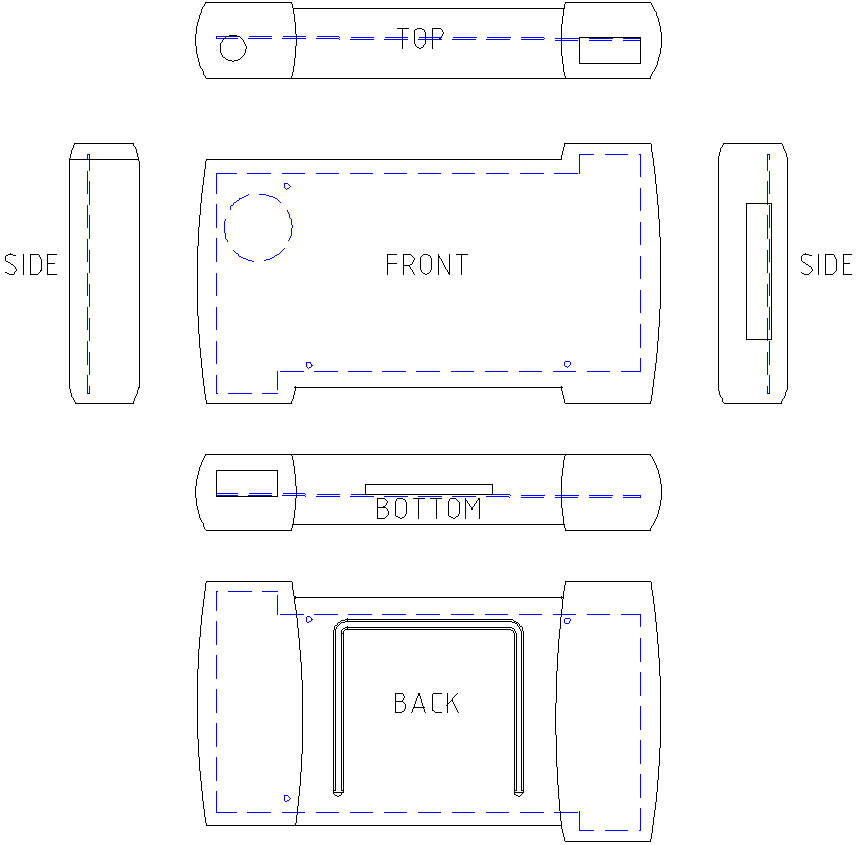
\includegraphics[width=10cm,height=10cm,keepaspectratio]{Figures/design1_sketch.png}
\caption{This is a sketch of the first concept design drawn to scale of the PCB}
\label{fig:Design_1}
\end{figure}

%-----------------------------------
%	SUBSECTION 2
%-----------------------------------
\subsection{Design Two}

The second design was intended to mimic a video game controller in order to conform better to the hand as well as give users a more intuitive layout in regards to the orientation of the device when in use. 
UD and the MEGAphone project have two common traits in that they intend for the device to be simple, to use and to defend against security threats under the mantra ‘security through simplicity’ REF. 
This concept inhabits this trait arguably to the highest degree.

\begin{figure}[hbt!]
\centering
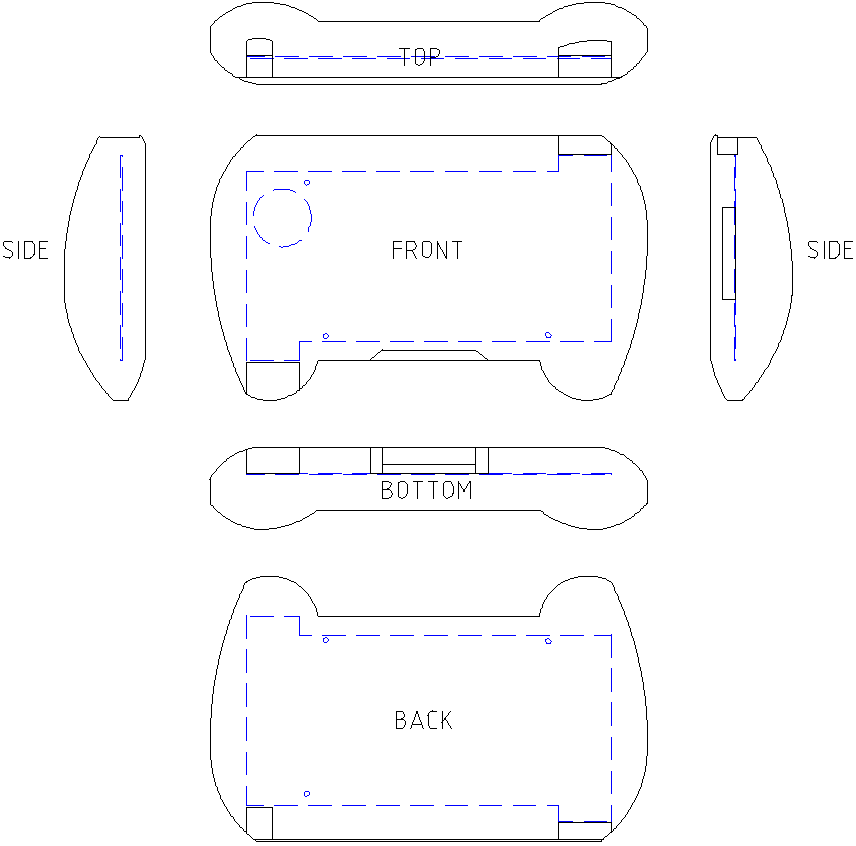
\includegraphics[width=10cm,height=10cm,keepaspectratio]{Figures/design2_sketch.png}
\caption{This is a sketch of the second concept design drawn to scale of the PCB}
\label{fig:Design_2}
\end{figure}

%-----------------------------------
%	SUBSECTION 3
%-----------------------------------
\subsection{Design Three}

There were a few factors that made this design the final candidate in which to base the main deliverable of this project.
This approach uses handgrips to subconciously hint to the user the correct orientation to hold the device.
The use of a stand to prop the device up for extended periods of time was a useful addition as it reduces the amount of effort from the user, therefore reducing fatigue.

\begin{figure}[hbt!]
\centering
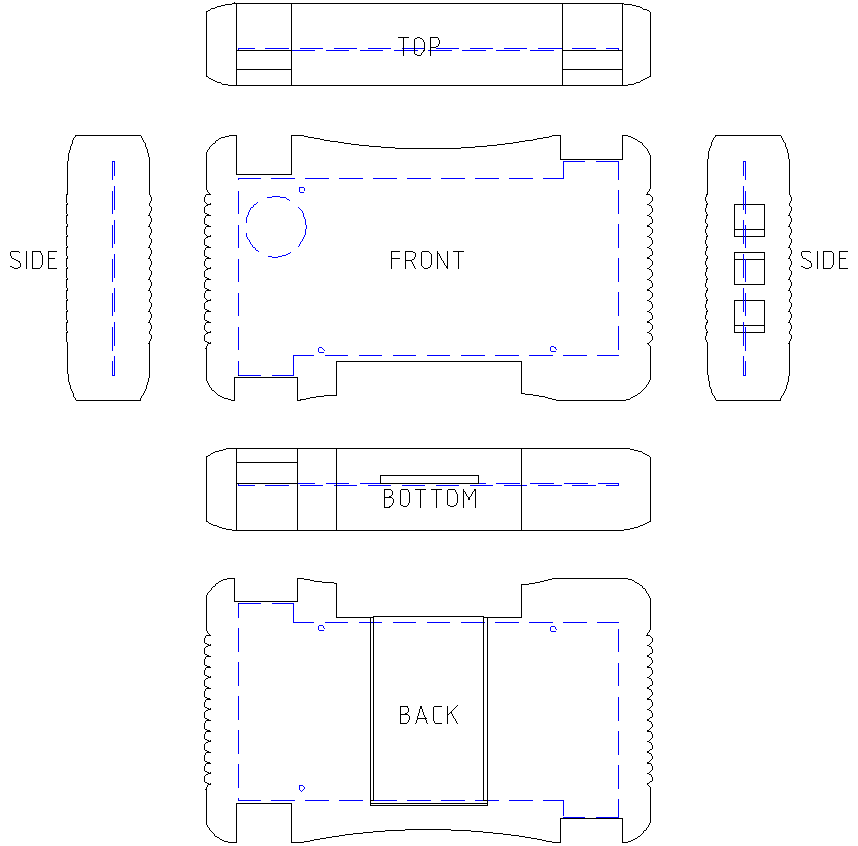
\includegraphics[width=10cm,height=10cm,keepaspectratio]{Figures/design3_sketch.png}
\caption{This is a sketch of the third concept design drawn to scale of the PCB}
\label{fig:Design_3}
\end{figure}

%----------------------------------------------------------------------------------------
%	SECTION 3
%----------------------------------------------------------------------------------------

\section{First Revision}

The following section covers the development of all aspects of the accessible MEGAphone chassis as well as the accompanying hardware such as buttons or hinges.

%-----------------------------------
%	SUBSECTION 1
%-----------------------------------
\subsection{CAD Sketch}

The first stage of design after the initial concepts was the CAD sketching stage.
This was approached by beginning with a front view of the sketch where users would typically interact with the device, however just the outline was extruded outwards in order to create a tangible object in which to mold and add features later on in the process.

%-----------------------------------
%	SUBSECTION 2
%-----------------------------------
\subsection{Hand Grips}

The first stage of design after the initial concept sketches intended to use rubber grips on both sides of the device featuring a ridged pattern.
However, this concept was removed in favour of a ridges that resemble the size and shape of human adult fingers to more intuitively direct the user to hold the device in the correct fashion as per design principle three.
Another aspect that was considered since the early stages, while less obvious in the final product due to the curved nature, was the introduction of rounded corners as this would minimise hazards to the user.
This was also the case with other edges of the device, in that they were filleted at 1.5mm to remove the sharpness of the device.

% This was after receiving feedback from my supervisor following an initial design (show design, before and after).

%-----------------------------------
%	SUBSECTION 3
%-----------------------------------
\subsection{Rocker Switches}

A major issue that was identified from the start with the second revision PCB was that placement and size of switches made it difficult to access.
Larger rocker switches were chosen to be placed on the front surface above the screen as this is in full visability of the user during use.
These switches relate to the security draw of the MEGAphone device, with insecure modules including, WIFI, bluetooth, two 4G modems, MEMS mics, LoRa radios and the FPGA serving as the central processing unit of the device.

The orientation of switches was completely intentional; for easier access for those with limited motor function or even without fingers, having the switches flip vertically would ensure that users are far less likely to flip wrong switch.
As well as this, the placement of these switches, above the display and away from other buttons on the device ensures that they do not interfere with the operation of the device.
Design principle one and three are satisfied by these rocker switches as they make the security features of this device easily available and the ON/OFF state of wireless modules is made abundantly clear (also supported by LED lights).

An earlier design incorporated the use of standoffs in the design in which to mount the PCB for the switches which was additionally included in the PCB design (view section 4.4). %fix this
This was however later removed due to not being necessary as when soldered to the switch contacts, the PCB would hold in place without issue and adding those supports would just add weight and increase complexity.

%-----------------------------------
%	SUBSECTION 4
%-----------------------------------
\subsection{Jellybean Switch}

The Jellybean switch bought exclusively for this project interfaces with the device using a 3.5mm Audio Jack connector. 
Given that it is a single digital input device, hardware-implemented accessibility capable of easily communicating with this device was relatively simple to implement. 
The second revision PCB during commencement of this project did not feature a working 3.5mm Jack connector, therefore, based on this knowledge, the 9-pin DSUB port of the device was hijacked as a single digital input under pin 7 for the Jellybean switch. 
The PCB ‘adapter’ created for this purpose is discussed in section 4.4. %fix this
This uses the same pin as the fire button on a retro Commodore64 Joystick controller, hence, integration into the MEGA65 operating system would be straightforward.

\begin{figure}[hbt!]
\centering
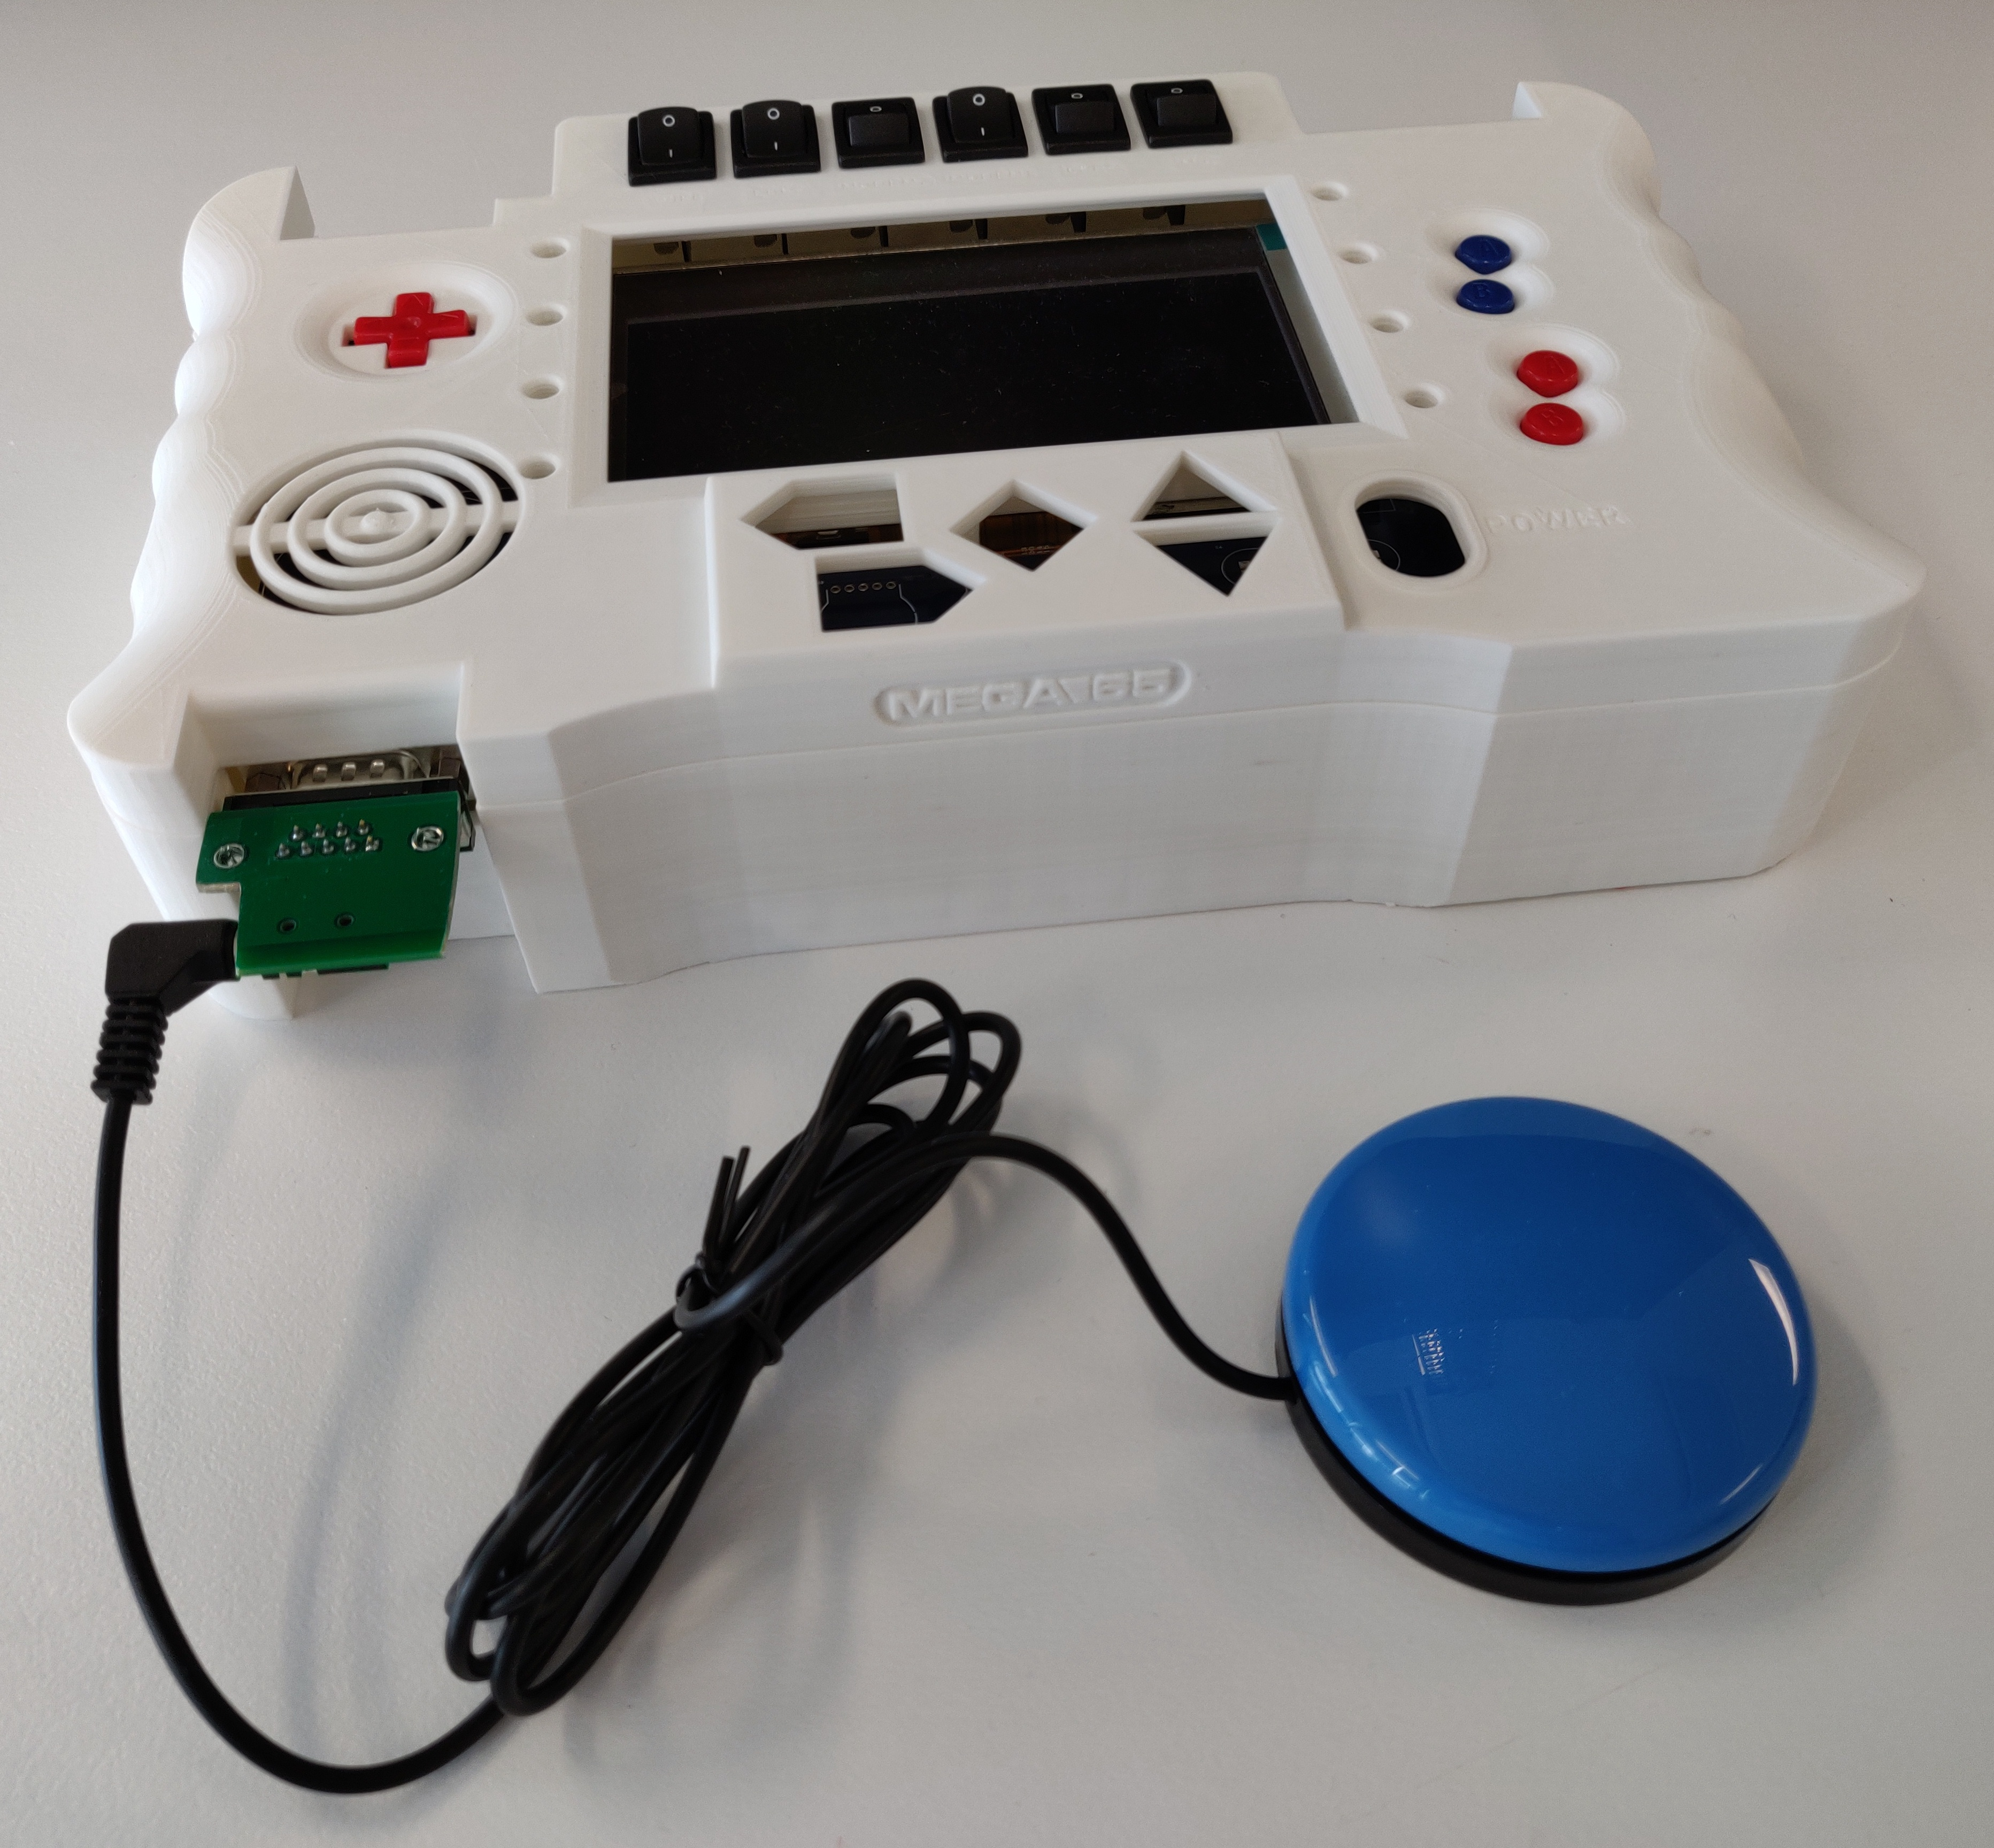
\includegraphics[width=10cm,height=10cm,keepaspectratio]{Figures/jellybean.jpg}
\caption{This is a physical example of how the Jellybean switch interfaces with the device during development}
\label{fig:Jellybean}
\end{figure}

%-----------------------------------
%	SUBSECTION 5
%-----------------------------------
\subsection{Recessed Buttons}

% talk about recessing the buttons so that if the device is dropped, minimal/no accidental button presses are registered
One concept that improves the ‘quality of life’ of this product was the addition of recessed buttons.
There are potential situations where the device might be accidentally dropped and unintended button presses may be recorded where the addition of recessed buttons avoids or at least significantly reduces the risk of this situation.
This feature also supports design principle five in that it minimises risks of unintended actions such as accidental button presses, which in this case would be if the user drops the device.

This feature is designed around another existing constraint in that the PCB uses buttons that were repurposed from spare Gameboy Advance parts. %%check this!
On the first prototype print, while allignment on the main MEGAphone PCB was correct, there was an issue regarding the clearance of the button cutout as well as the positioning of slots to hold the buttons in the correct orientation.

%-----------------------------------
%	SUBSECTION 6
%-----------------------------------
\subsection{3D-printed Prototype}

There was a significant issue that was overlooked with the first 3D printed prototype in that the thought behind orientation of components was flipped.
Electronic components (including connectors) needed more space underneath in order to fit comfortably and the design up until that point had not properly accounted for it.
The biggest issue was that the device ports were initally not thought of in the correct orientation.
The orientation of these ports is very important as this dictates how much volume each of the two main case components takes.
To rectify this issue, 

% so explain the process of rectifying this issue, map out the impacts and how they are resolved
% also add in that 0.15mm print resolution was used, not perfect as the project was very precise on top case in some parts, such as buttons, hence this should be done at higher resolution which means longer print time or silicone injection mould as a likely stronger, neater alternative

%-----------------------------------
%	SUBSECTION 7
%-----------------------------------
\subsection{Device Stand}

% thoughts behind the device stands, how they were conceptualised and why it was approached in such and such way; having two stands on either side adds to stability of the device as opposed to the original idea of having one stand in the middle, which also leaves space for solar panel in the middle
Originally the approach was to have a single stand oriented in the middle of the device where users could extend it out as they need.
However, having two stands on either end of the device has multiple advantages in that doing so increases the stability of the device, as well as gives ample space in the centre to place one or multiple solar panels depending on the available space (discussed in section 3.8).
The mechanism in which to extend and 'lock' the stand in place had the potential to be approached from a number of different angles.
One such angle that was a part of the final prototype was to have a sliding..

%%add trigonometric function to determine angle of stand 'foot'

%-----------------------------------
%	SUBSECTION 8
%-----------------------------------
\subsection{Solar Panels}

% choice of solar panels, discuss potential options and why a specific one was chosen, do a table comparison of available panels and again explain the power output and cost etc.
Giving users more ways to charge their device plays heavily into the digital sovereignty aspect of this project.
A number of solar panels from two suppliers (Digikey, Mouser) were analysed based on cost, size and energy output for a designated area set out on the MEGAphone case at 125mm by 140mm, collated in figure X.

\begin{center}
    \begin{tabular}{ |c|c| } 
    \hline
    cell1 & cell2 \\
    \hline
    cell1 & cell2 \\ 
    \hline
    cell1 & cell2 \\ 
    \hline
    cell1 & cell2 \\
    \hline
    \end{tabular}
\end{center}

\begin{figure}
    \caption{An analysis of various solar arrays and their suitability to a designated space on the MEGAphone chassis}
    \label{fig:DesignPrinciples}
\end{figure}

%-----------------------------------
%	SUBSECTION 9
%-----------------------------------
\subsection{Device Strap / Key-chain}

% talk about process of designing this feature, how original design changed in favour of larger slot/strap for easier carry
The thought behind the key-chain feature of the device was to be able to clip it to something or alternatively fix items to it, and while this feature did see an appearance in an early prototype, it was later adapted into a 'housing' for an arm strap, to allow for easier carrying as this was considered to be more useful.
The reasoning for this was that a key-chain feature would not have many practical applications in terms of hanging items off of it, and so the introduction of a much larger opening to integrate a carry strap would better benefit design principle six as it would distribute the weight of the device more evenly when carried.
Another consideration was the addition of an extra notch, added to lock into the top part of the case and re-enforce the strength as the entire weight of the device would otherwise be supported by one end of the slot. %%revise, find better name for 'slot'

%-----------------------------------
%	SUBSECTION 10
%-----------------------------------
\subsection{Easy Access Keys}

The easy access keys or 'EZ Keys' were inspired by the 'Nav Keys' developed by Storm Interface [source] which feature an array of easily distingishable keys which were inspired for this adaptation.
These keys benefit from being easily perceptible, due to each button having a unique colour and shape, which envelops the forth design principle.

The EZ Keys were first approached as an extension of the device as this would free up a lot of the limited space available.
This would mean making a separate housing and having the device plug into the 9pin DSUB port similarly to how the Jellybean switch (see section 3.4) would interface with the device.
It was ideal for the array of buttons to be integrated into the device as this ensures that the full extent of accessibility is available from the moment the device is picked up.

Due to the height requirement of the MEGAphone PCB, there was very little space to attach a slave PCB to allow button functionality, hence one of the reasons why there is an elevation in the button housing.
The second reason for there being an elevation in the EZ key setup is due to the desire to make it more perceptible (design principle four) to users as the position of the power button nearby meant that it would be important to ensure that users do not accidentally press the wrong button (design principle five).
Additionally, there needed to be enough depth so that the PCB could be screwed into place comfortably, elevated slightly above the main MEGAphone PCB as there would be an overlap due to the size and shape of both PCBs.

An issue that came up in the first prototype print is that the keys did not have enough clearance to actuate without resistance, also in common with the A, B and directional buttons.
This was fixed in an update by extending the width of the button cutouts by approximately 0.3mm as this would also theoretically align with the 0.15mm print resolution. % check this

% FIXED AB AND DIRECTIONAL BUTTON SIZE CLEARANCE, ALSO EZ KEY CLEARANCE
% FIXED ALIGNMENT OF THROUGH HOLE

%-----------------------------------
%	SUBSECTION 11
%-----------------------------------
\subsection{Ventilation} %PROBABLY CHAPTER 5

% device only uses about 1-2W of power, FPGA using 0.2W
% Not necessary in final design but add images of version with vents
Thermal management is a concept that came up later in the process as the MEGAphone device is a low power device by mobile device standards.
In its entirety, the device uses approximately 1-2W of power with the heart of the device, the FPGA, using about 0.2W of power.
This yields very little thermal output with the more notable power drawing components being the 110db speaker [source] and full colour 480p display [source].

%-----------------------------------
%	SUBSECTION 12
%-----------------------------------
\subsection{Potentiometers}

% Slide pot better than thumb wheel pot, explain about physical effort etc.
%% LIKELY GOING IN CHAPTER 5
The potentiometer feature used to control aspects such as speaker volume was a feature that was omitted from the final design due to another more important requirement being the implimentation of EZ keys.
This is a feature that can be implemented by other means such as through the EZ keys themselves and therefore a prototype without this would not be a major issue.
The best solution for this would be to employ an array of sliding potentiometers to control any desired functions such as volume control, as pertaining to design principle six, would be the easiest in terms of the amount of effort that users have to extert.
Any potentiometer that is too small or requires a twisting motion would be more difficult for some users, such as elderly users with a weaker grip strength.

%-----------------------------------
%	SUBSECTION 13
%-----------------------------------
\subsection{Port Access}

Port access was intentionally designed to have no case material on the top and bottom of the device minimise interference with the plugging in of various peripherals, supporting design principle seven.
These ports are all labelled, explaining in one word the purpose of each port to make it abundantly clear to the user.

An issue that was faced in the original prototype was in regard to the orientation of the port cutouts that were placed on the display side of the PCB.
This was rectified by extending out the bottom chassis component with the port cutout on that side so that it would match up with the true orientation of the ports. %expand on this later with images

%-----------------------------------
%	SUBSECTION 14
%-----------------------------------
\subsection{Threaded Inserts}

An important aspect of this deliverable is to have a method of securing all parts in place as well as being easily accessible to users who which to repair or modify certain aspects.
This means using parts that are not obsecure such as a 'pentagon star' screw[REF], where users would typically not have the suitible screwdriver for that job.
Naturally, this would all be fastened using 'phillips head' screws as these are widely considered the most common screw head type aside from 'flat head' screws.

These constraints were already set out for the MEGAphone PCB in that there are holes in certain parts of the case for this exact purpose.
However, an issue that had to be addressed was the placement of certain components on the PCB and their vicinity to these 'mounting' points.
In particular, one of the MEMs mics, some resistors and transistors were placed closer to this mounting point than what would've been ideal and for this reason, certain parts of the mounting supports were trimmed around these obstacles.

The choice to use threaded inserts for this project was due to its reliability, in that the threads must be consistent due to strict manufacturing standards.
The alternative that would acheive the same outcome would have been to 3D print solid standoffs and use self-tapping screws in order to securely fasten the device.
This option is however more unreliable as it requires user guided input, a reasonably soft material to be effective and most importantly would require a 100 percent 3D infill, almost doubling the overall print time.
A third option that was diregarded would have been to 3D print the threads, which at a 0.15mm print profile, would have left much room for error considering that this project requires considerably small M3 screws to remain compliant with the constraints of the MEGAphone PCB.

%----------------------------------------------------------------------------------------
%	SECTION 4
%----------------------------------------------------------------------------------------

\section{PCB Design}
This section discusses the process in designing the supporting PCBs for this project.
% explain workaround for previous button layout, using slave boards with tactile switches as well as choice behind contact pads instead of connectors to save space

%-----------------------------------
%	SUBSECTION 1
%-----------------------------------
\subsection{Rocker Switch PCB}

The PCB designed to organise the routing of power to the array of rocker switches originally had the intention of interfacing with the main PCB through a connector of some sort.
With space being a limited factor, an alternate solution was carried out.
The introduction of 'mounting' pads to serve as a soldering point for the wires would allow them to be comfortably routed to the main PCB.

An issue with the footprint that was observed after sourcing these parts, was that there was not enough clearance for the pins to 'slot' through.
The approach was to file down the pins on the rocker switches individually so that they would fit, which was not an issue in regards to current as the whole device runs on about 1-2W, with a rocker switch[REF] able to handle approximately 2kW of alternating current.
Filing down the PCB through-hole cutout would have made for a far worse alternative as there was potential for solder to not flow evenly due to damaging the solder mask. %double check this

During the case design process, having mounting points to hold the circuit board in place was implemented.
This was later removed as the switches mount very securely in their cutouts coming from a top-down orientation and so pressing in or flicking these switches would not put any stress on the PCB, unlike the EZ keys in section 4.2.
Doing so allows for adjustment if needed before soldering as well as less parts making the repair process easier if users need to replace or modify certain parts.

Clearance between the PCB and the main MEGAphone PCB was additionally very minimal and so the introduction of a bulky connector would make containment of this device far more difficult.
An alternative to this that would have proven effective and arguably neater in a final version would have been to employ the use of a low profile 'ribbon' style connector with separate wires that are thick enough to handle decent current as well as be indepenently wired to different areas of the MEGAphone PCB.
The reason why this was not chosen is because this deliverable is a proof of concept where the intention is for the MEGAphone PCB to be redesigned so that these rocker switches can be incorporated into the main design, therefore purchasing these connectors for this purpose would be ultimately wasteful.

%-----------------------------------
%	SUBSECTION 2
%-----------------------------------
\subsection{Easy Keys and Power}

The purpose behind the easy keys is to give users a platform in which to interact with the MEGAphone device while being as clear and easy to use as possible.
Multi-coloured, multi-shaped keys are employed make things as unambiguous as possible which include, left and right (forward and backward), up and down, and a 'fire' or enter key.
This, as discussed in section 3.10, is inspired by the Storm Nav-pad[source], where a version has been acheived to a budget, for the purpose of prototype development.

An important aspect of this device is to provide easy access to the power switch as turning the display on an off on this device is frequent due to not having automatic display toggle features.
This is intergrated into the device in the same manner as the easy keys, in that they work by momentarily pressing a tactile switch.
These tactile switches are wired directly to the GPIO expander linked to the FPGA on the MEGAphone PCB with the idea being that this new external PCB serves as an extension of the main board.

This interface faced an issue where the openings for the button cutouts were virtually the same size leading to problems with clearance. 
To fix this issue, the openings were extended by about half a millimetre on all sides to allow for smooth button pressing while still sitting securely in place.

%-----------------------------------
%	SUBSECTION 3
%-----------------------------------
\subsection{Audio Jack Adapter}

The audio jack adapter was designed to be a substitute for the original audio jack setup fully integrated on the MEGAphone PCB, which was unoperational at the time.
This PCB hijacks the fire pin of the 9-pin DSUB connector in order to 'imitate' a joystick fire button. 
Coupled with hardware implemented features in the FPGA, the MEGA65 OS should treat this input as a regular peripheral such as a joycon.

An issue that was faced during the course of development regarded the overall size and shape of the PCB.
This was not thought about correctly at the time of manufacturing as the PCB was too bulky on either side.
Additionally, due to the central placement of the audio jack input and the bulky Jellybean switch jack output, interfacing with this adapter was less than convienient.
To fix this, a nibbler was used to clip away at the edges to cut the board down to size, followed by a rough 80 grit sanding to smooth the edges somewhat.
Given that fibreglass particles are not good for health when inhaled, this was undertaken responsibly to ensure that these risks were avoided.


%----------------------------------------------------------------------------------------
%	SECTION 5
%----------------------------------------------------------------------------------------

\section{PCB Layout}  %% THIS WILL PROBABLY BE CHAPTER 5

% analyse the changes in the final design, what limitations the existing PCB layout has and propose a better layout that satisfies the UD principles, talk about what is ideal and what is the best that can be done with current layout. 
% Ideal layout includes ports at top of device along with rocker switches replacing current rev2 switches on the main PCB

%-----------------------------------
%	SUBSECTION 1
%-----------------------------------
\subsection{Original Design}

The layout of the second revision MEGAphone PCB served as the major constraint of this project, as the case design had to be designed around it without any significant redesign due to the complexity of the device. 
Certain reworks to better adapt the design to an accessible interface included removing the existing switches in favour of larger rocker switches hosted on an external PCB (view figure).

%-----------------------------------
%	SUBSECTION 2
%-----------------------------------
\subsection{Proposed Design}

A possible solution to the existing PCB which does inhabit the Universal Design principles is proposed in FIGURE. 
The underlying idea with this redesign was to integrate the design all onto one PCB. 
Doing so would reduce the amount of wires required and given that those in the current solution are soldered to make space, it makes the design overall ‘simpler’.

In order to make the device more intuitive, placement of the 9-pin DSUB port should be moved to the ‘top’ of the device in the same orientation as the VGA port, so that users know from a glance that this is where all device ports are expected to be.
The accessible button interface also utilises an external PCB which hosts the tactile switches that were opted to form the base of the accessible button function. 
Other options were considered, such as silicone rubber pads, as used for the directional button and ‘A’, ‘B’ buttons. 
However, primarily due to the size, larger buttons would be recommended as this would make button presses easier for all users, disregarding the EZ keys in this scenario.

%----------------------------------------------------------------------------------------
%	SECTION 6
%----------------------------------------------------------------------------------------

\section{Software Accessibility}
% talk about keyboard accessibility, term ‘android accessibility encapsulation’ discuss this.
% Also mention program is working in parallel to the software ‘mimicking’ the c64 system so this is not a C program running on MEGA65 but rather VDHL, a hardware description language
Keyboard 'software' accessibility goes hand-in-hand with the Jellybean switch input (view section 3.4) as this is primarily what is used to control this feature, aside from the potential to implement this on an EZ key button by hijacking the same pin.
This is all hardware-implemented in the FPGA, with the intention of being completely transparent to the MEGA65 operating system.
This means that the accessible keyboard runs in parallel to the operating system and therefore should not 'see' the Jellybean switch, but instead treat it as if it were any peripheral, such as a Commodore64 joycon[source].
Due to the Jellybean switch being a simple digital input device, this made implementing this feature relatively straightforward.

%-----------------------------------
%	SUBSECTION 1
%-----------------------------------
\subsection{Accessible Keyboard Framework}
//

%-----------------------------------
%	SUBSECTION 2
%-----------------------------------
\subsection{Accessible Interface}
//

%----------------------------------------------------------------------------------------
%	SECTION 7
%----------------------------------------------------------------------------------------

\section{Summary}
// 
% Chapter Template

\chapter{Conclusions and Future Work} % Main chapter title %% EXTRACT RESULTS SECTION FROM HERE TO NEW CHAPTER

\label{Chapter5} % Change X to a consecutive number; for referencing this chapter elsewhere, use \ref{ChapterX}

%----------------------------------------------------------------------------------------
%	SECTION 1   % TARGET 1500 WORDS IN THIS CHAPTER
%----------------------------------------------------------------------------------------

\section{Overview}
This chapter provides concluding remarks on the deliverables of chapter 4 and provides a discussion on aspects where the project would benefit moving forward.

%----------------------------------------------------------------------------------------
%	SECTION 2
%----------------------------------------------------------------------------------------

\section{MEGAphone Chassis/Case First Revision}
The MEGAphone accessible chassis project was fully realised on the 8th of November, 2020. 
In this chapter, the development of the project and how various aspects benefit the usability of the MEGAphone device as a whole, will be analysed. % maybe add to overview
Additionally, a discussion on the potential future work of the project will establish how to best approach a succeeding revision of the chassis and the MEGAphone PCB followed by some concluding remarks. \newline

This thesis has answered the following research questions in the preceding chapters:
\begin{enumerate}
    \item What is the relationship between Digital Sovereignty and Universal Design?
        \begin{enumerate}
        \item[-] ...
        \end{enumerate} 
    \item Why is Universal Design important in the design of products today?
        \begin{enumerate}
        \item[-] ...
        \end{enumerate}
    \item Why is Digital Sovereignty important in the design of electronic products today?
        \begin{enumerate}
        \item[-] ...
        \end{enumerate} 
    \item How can the seven design principles be used in the design of the MEGAphone case to support those with disabilities?
        \begin{enumerate}
        \item[-] ...
        \end{enumerate} 
    \item How can the 'Right to Repair' mantra be used in support of the universally designed MEGAphone case?
        \begin{enumerate}
        \item[-] ...
        \end{enumerate} 
    \item What are the effects of COVID-19 on Digital Sovereignty, Universal Design and the MEGAphone project?
        \begin{enumerate}
        \item[-] ...
        \item[-] ...
        \end{enumerate} 
\end{enumerate}

% %-----------------------------------
% %	SUBSECTION 1
% %-----------------------------------
\subsection{Subsection 1}
//

% %-----------------------------------
% %	SUBSECTION 2
% %-----------------------------------
\subsection{Subsection 2}
//


%----------------------------------------------------------------------------------------
%	SECTION 3
%----------------------------------------------------------------------------------------
\section{Future Work}
The following section addresses both the MEGAphone PCBs and the accessible chassis with a discussion on the recommendations of the project moving forward.

%-----------------------------------
%	SUBSECTION 1
%-----------------------------------
\subsection{Original PCB Layout}
% analyse the changes in the final design, what limitations the existing PCB layout has and propose a better layout that satisfies the UD principles, talk about what is ideal and what is the best that can be done with the current layout. 
% Ideal layout includes ports at top of device along with rocker switches replacing current rev2 switches on the main PCB
The layout of the second revision MEGAphone PCB served as the major constraint of this project, as the case design had to be designed around it without any significant redesign due to the complexity of the device. 
Certain reworks to better adapt the design to an accessible interface included removing the existing switches in favour of larger rocker switches hosted on an external PCB (view figure).

\begin{figure} [h]
\begin{centering}
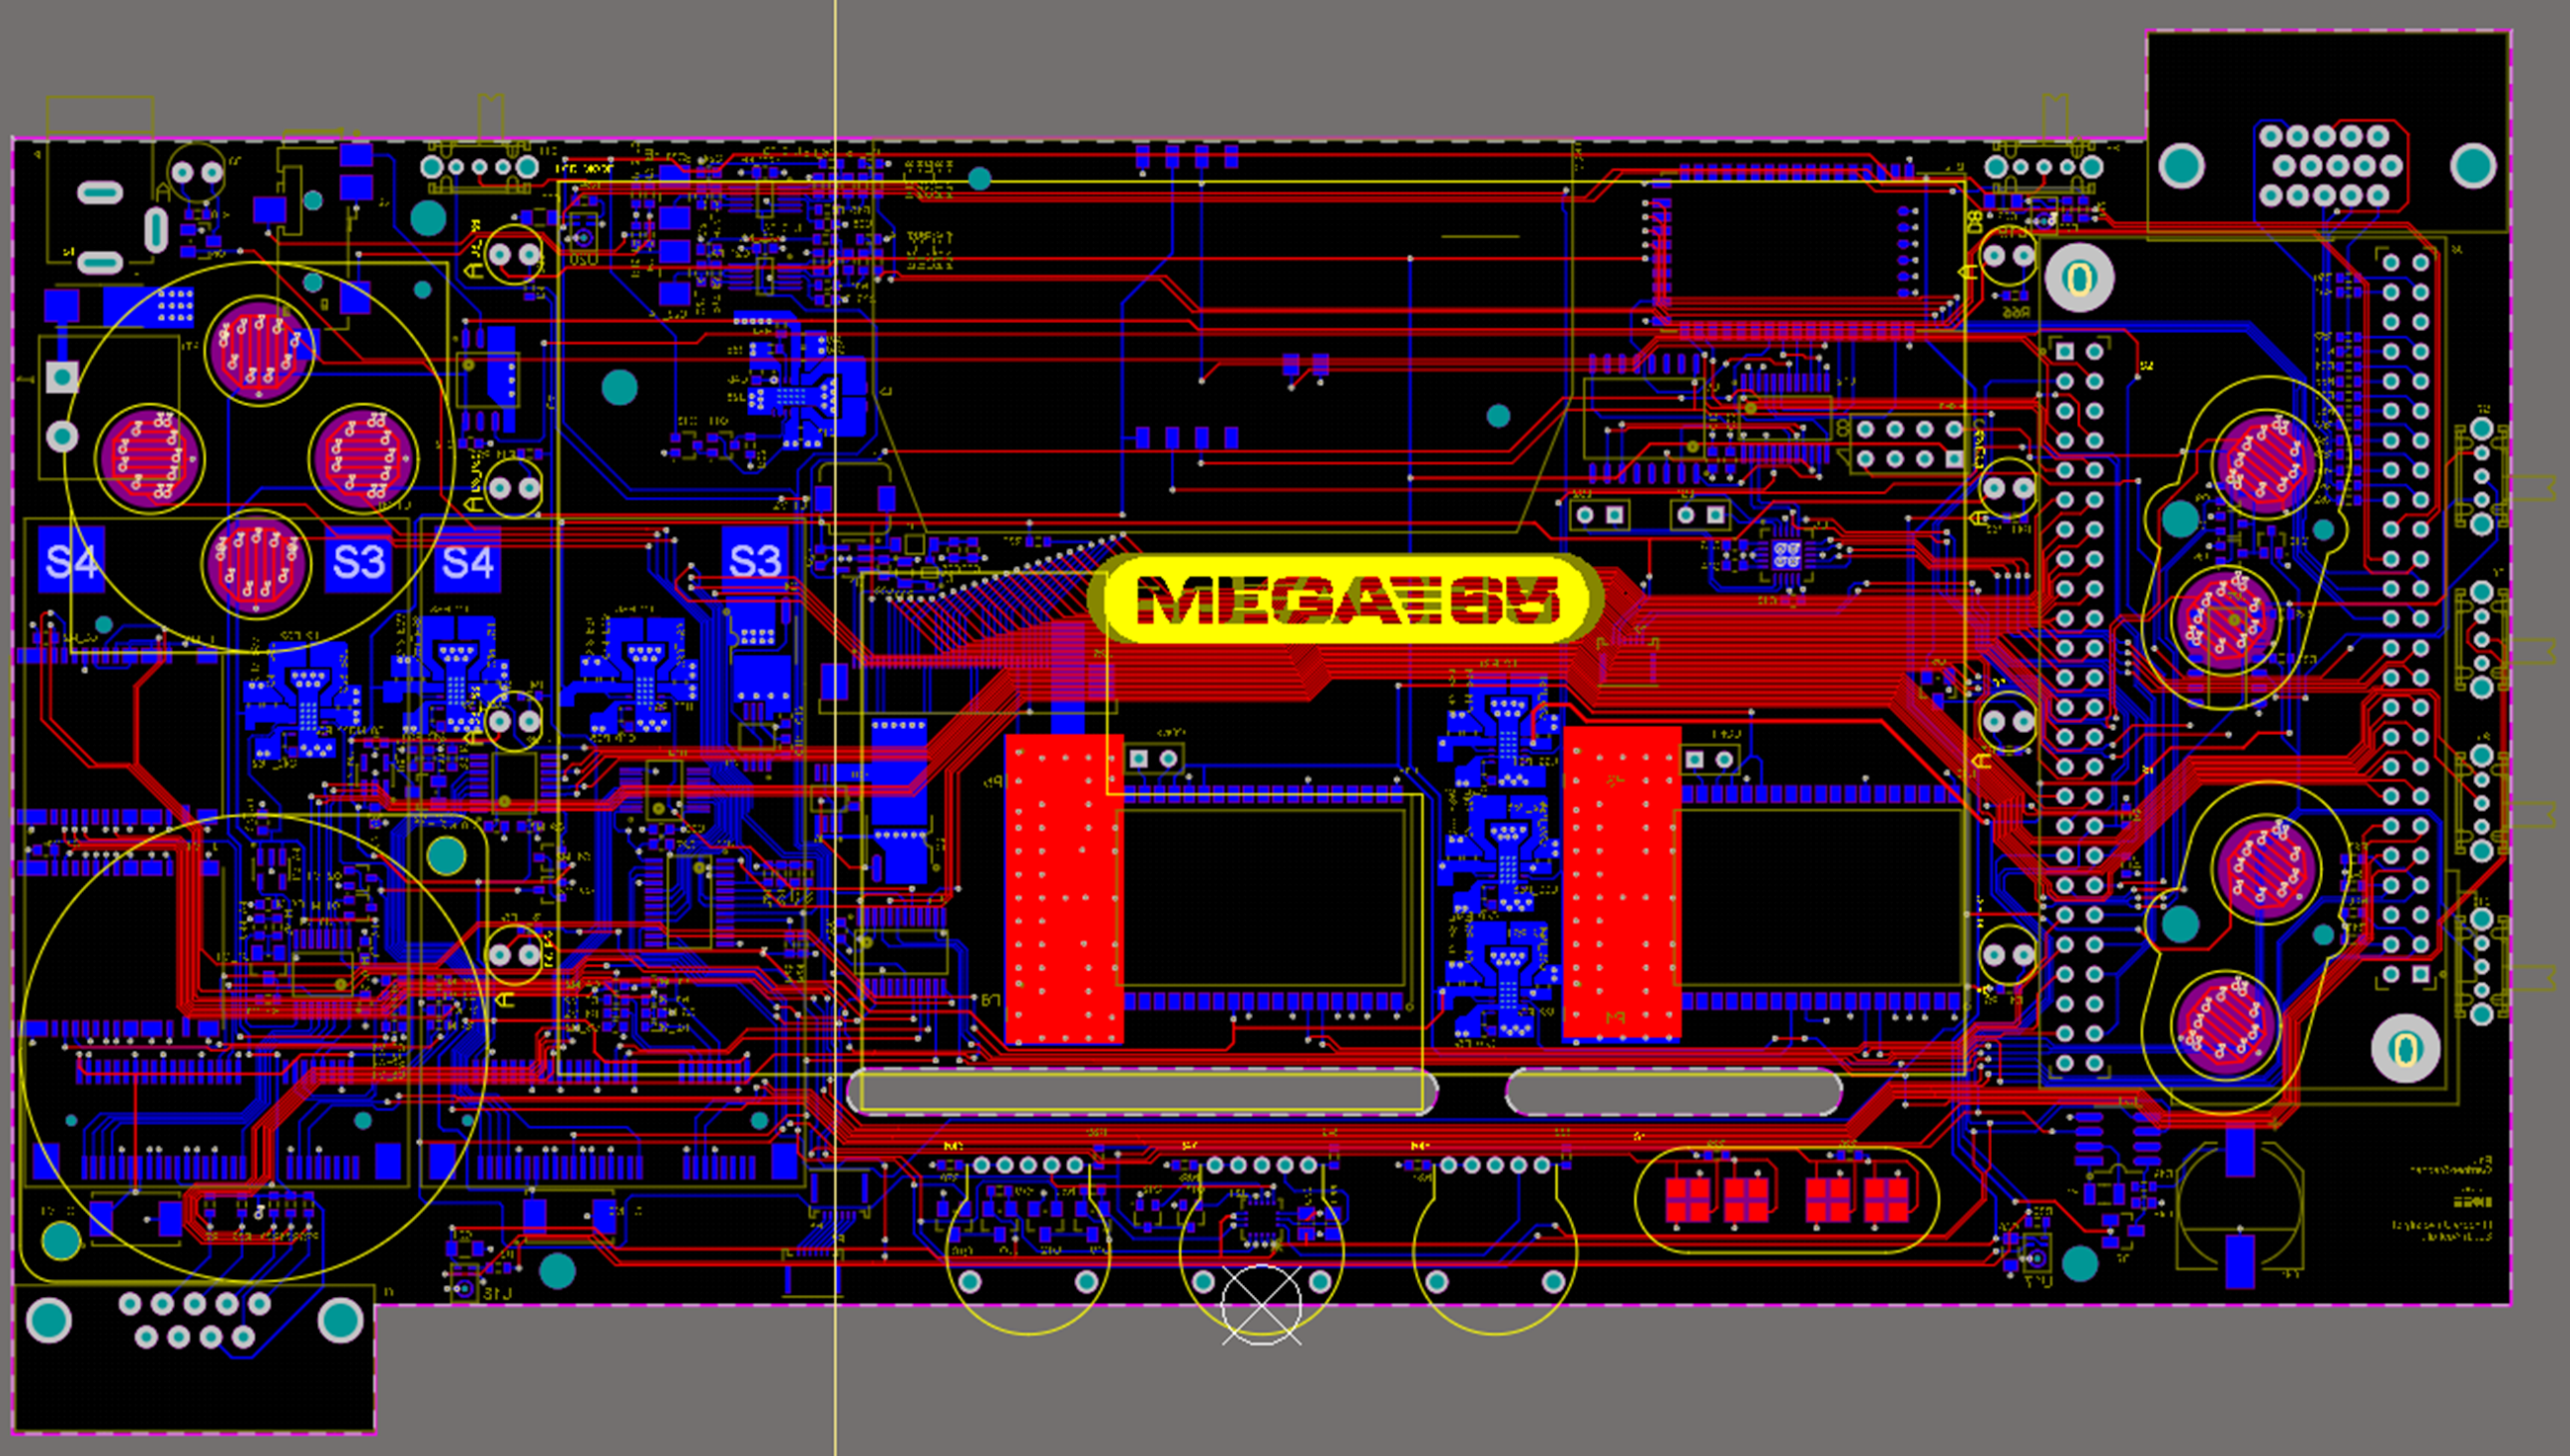
\includegraphics[width=10cm,height=10cm,keepaspectratio]{Figures/pcb_original.png}
\caption{This is the PCB layout as it was during the development of this project.}
\label{fig:ThisFig}
\end{centering}
\end{figure}

%-----------------------------------
%	SUBSECTION 2
%-----------------------------------
\subsection{Proposed PCB Layout}

A possible solution to the existing PCB which does inhabit the Universal Design principles is proposed in figure X. 
The underlying idea with this redesign was to integrate the design all onto one PCB as doing so would reduce the quantity of wires required and given that those in the current solution are soldered to make space, it makes the design overall ‘simpler’.
The reason for the redesign not being undertaken in this project has been discussed previously as impractical due to an issue of cost and time.

\begin{figure} [h]
\begin{centering}
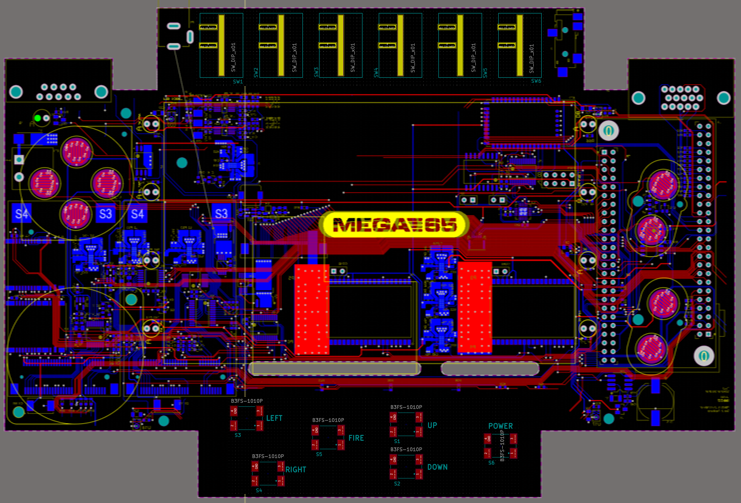
\includegraphics[width=10cm,height=10cm,keepaspectratio]{Figures/pcb_final.png}
\caption{This is the PCB as it is proposed in a future revision of the MEGAphone project.}
\label{fig:ThisFig}
\end{centering}
\end{figure}

In order to make the device more intuitive, placement of the 9-pin DSUB port should be moved to the ‘top’ of the device in the same orientation as the VGA port, so that users know from a glance that this is where all device ports are expected to be.
The accessible button interface also utilises an external PCB which hosts the tactile switches that were opted to form the base of the accessible button function.

Other options were considered, such as silicone rubber pads, as used for the directional button and ‘A’, ‘B’ buttons. 
However, primarily due to the size, larger buttons would be recommended as this would make button presses easier for all users, disregarding the EZ keys in this scenario.
It is acknowledged that larger buttons on the PCB would invalidate the current Gameboy buttons, which is why a complete redesign of those buttons would be recommended to further progress the accessibility of the device as a whole.

It is also recommended that the device incorporates multiple 3.5mm jack inputs, separate from the audio function, in its design as this can give users the ability to plug in multiple switches much like the Jellybean presented in this project.
Microsoft's accessible controller \cite{adaptive} is a prime example of the usefulness of this feature and for those who might not be able to interact with the EZ keys or Gameboy buttons but desire their means of interaction with the device, multiple inputs allow for multiple unique functions.
Placement of these inputs should be at the 'top' of the device with all other ports as can be seen in figure X, as this minimises complexity by ensuring that everything is in one place for the user.

%----------------------------------------------------------------------------------------
%	SECTION 4
%----------------------------------------------------------------------------------------

\section{Final Summary}
// 

%----------------------------------------------------------------------------------------
%	THESIS CONTENT - APPENDICES
%----------------------------------------------------------------------------------------

\appendix % Cue to tell LaTeX that the following "chapters" are Appendices

% Include the appendices of the thesis as separate files from the Appendices folder
% Uncomment the lines as you write the Appendices

% Appendix Template

\chapter{Inital Concept Designs} % Main appendix title

\label{AppendixA} % Change X to a consecutive letter; for referencing this appendix elsewhere, use \ref{AppendixX}

\clearpage

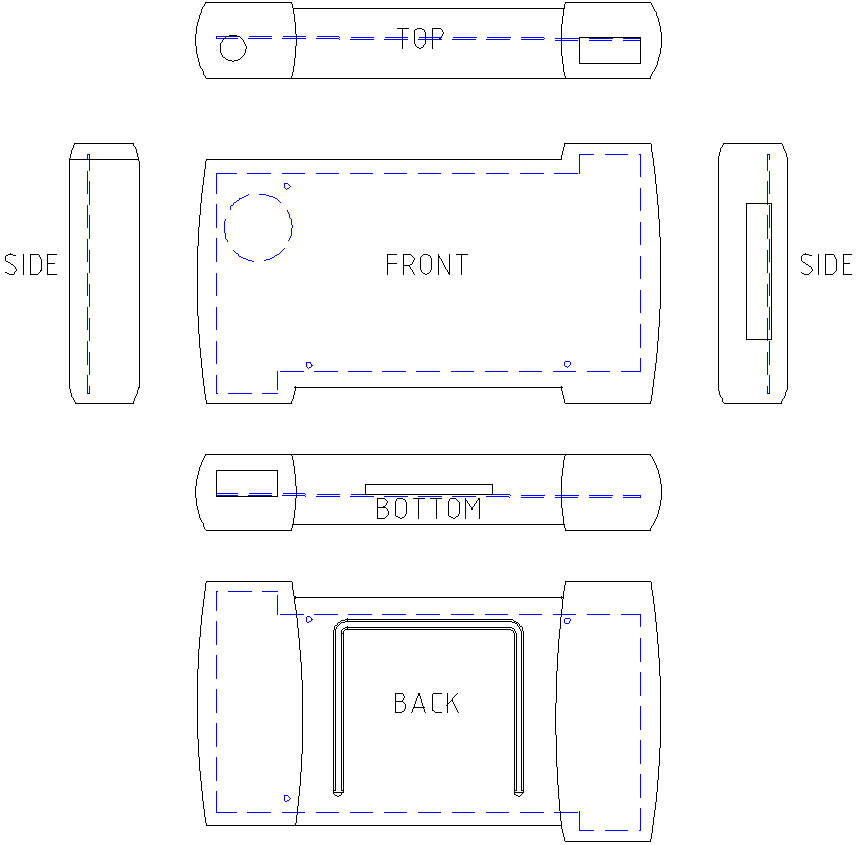
\includegraphics[width=14cm,height=23cm,keepaspectratio]{Figures/design1_sketch.png} \newline

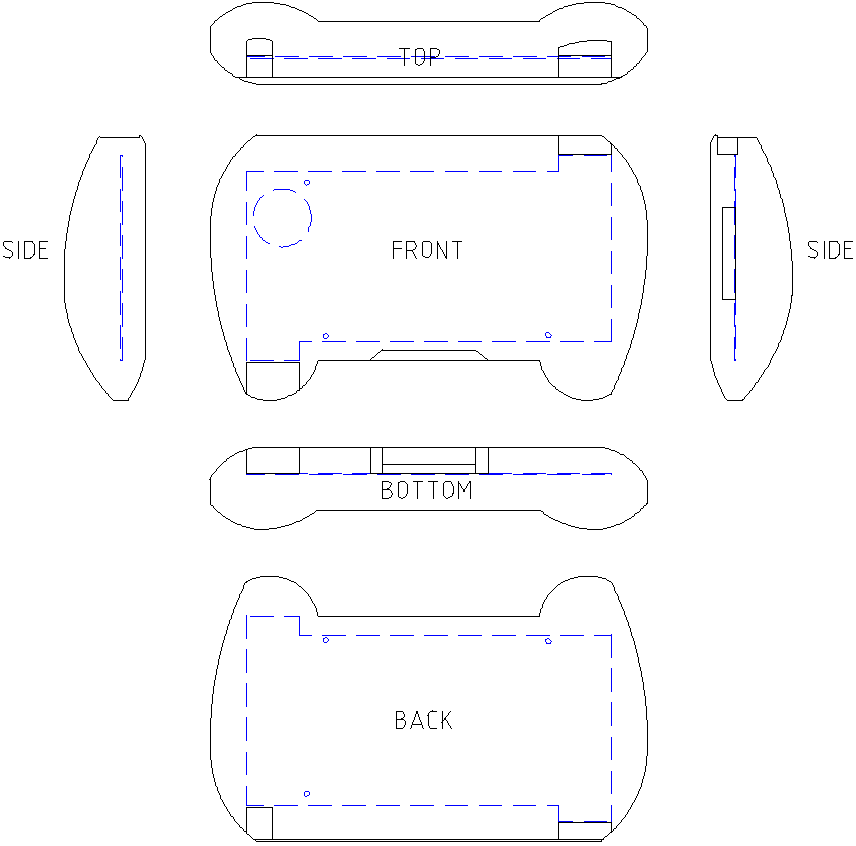
\includegraphics[width=14cm,height=23cm,keepaspectratio]{Figures/design2_sketch.png} \newline

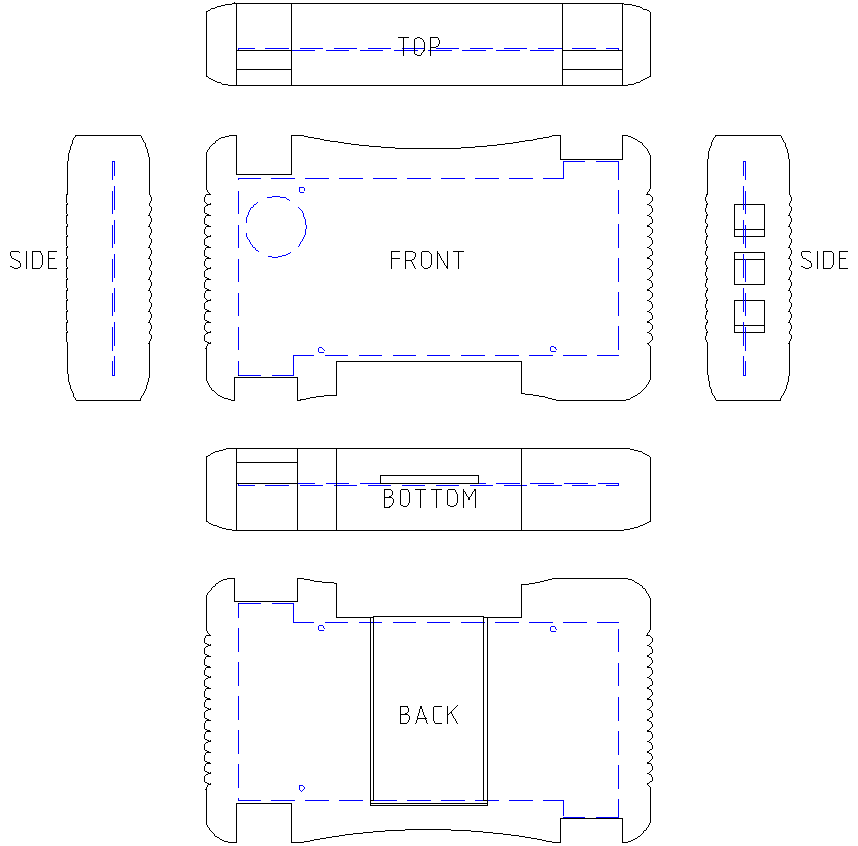
\includegraphics[width=14cm,height=23cm,keepaspectratio]{Figures/design3_sketch.png}

%% Appendix Template

\chapter{Printed Circuit Board Designs} % Main appendix title

\label{AppendixB} % Change X to a consecutive letter; for referencing this appendix elsewhere, use \ref{AppendixX}

Write your Appendix content here.
%% Appendix Template

\chapter{MEGAphone CAD Iterations} % Main appendix title

\label{AppendixC} % Change X to a consecutive letter; for referencing this appendix elsewhere, use \ref{AppendixX}

\clearpage

\section{First Iteration}
//
\newpage

\section{Second Iteration}
//
\newpage

\section{Third Iteration}
//
\newpage

\section{Forth Iteration}
//
\newpage

%----------------------------------------------------------------------------------------
%	BIBLIOGRAPHY
%----------------------------------------------------------------------------------------

\printbibliography

\end{document}